\documentclass[11pt]{article}
\usepackage[margin=1in]{geometry}
\usepackage{graphicx,booktabs,amsmath,amssymb,url,microtype}
\usepackage[numbers,sort&compress]{natbib}
\usepackage[hidelinks]{hyperref}
\graphicspath{{figs/}}
\renewcommand{\topfraction}{0.95}\renewcommand{\bottomfraction}{0.6}\renewcommand{\textfraction}{0.05}\renewcommand{\floatpagefraction}{0.85}\setcounter{topnumber}{3}\setcounter{totalnumber}{4}
\setlength{\textfloatsep}{9pt}\setlength{\intextsep}{8pt}\setlength{\abovecaptionskip}{4pt}\setlength{\belowcaptionskip}{2pt}
\newcommand{\rid}[1]{{\footnotesize\texttt{#1}}}
\title{Steered affect moves a conversational partner's activations:\\ the estimator, three pre-registered ablations, and the controls register}
\author{Manan Wadhwa\thanks{Revised draft of 2026-09-06 after three adversarial reviews, a mentor review, a citation audit and a statistical-consistency audit (all in the repository). Every number is registered in \texttt{docs/review/claims.json} under the identifier printed after it in monospace; the registry is machine-checked against the result files. Figures and tables are generated from those files by \texttt{src/rev3/paper\_figures.py} and \texttt{src/rev3/paper\_revision\_stats.py}.}}
\date{}
\begin{document}
\maketitle

\begin{abstract}
When one language-model agent is steered into an emotion and talks to another, a linear probe's projection of the second agent's reply activations moves with the dose, for five of six emotions on Qwen3.6-27B and on Llama-3-8B. We ask what carries it, and find that the standard linear tools mislead in ways their usual checks do not catch. The logistic-regression direction most work uses to read and write such states reproduces across disjoint halves at only 0.57 (27B, $n=2000$ per half) and 0.29 (8B), while difference-of-means reaches 0.97 and 0.94 on the same splits, and a fixed per-sample penalty does not close the gap. In the $n<d$ regime probe studies work in, every logistic fit is a perfect separator: its direction is the penalty's tie-break, drifting from the mean difference as $n$ grows (cosine 0.97 to 0.63); projected onto 100 principal components, where $n \gg d'$, the fits stop separating and the direction reproduces at 0.90. The cost is largely geometric: the two estimators' held-out projections correlate at 0.90--0.96. With the reproducible direction, three pre-registered ablations test the linear account of the channel. Removing the emotion direction at every readable layer leaves a median 91\% of the response, against a random-direction control or against baseline (83\% with the untestable emotion included); a rank-5 affect subspace fails its own instrument check; a rank-5 subspace fitted by the same estimator on permuted labels blocks three emotions as strongly as the affect subspace does, while a random 5-frame of half its footprint, a random 23-frame of the same footprint and a permuted-label rank-1 direction are inert. Re-estimating every direction on ten re-splits of the probe pool, the emotion direction's block of sad against the permuted control holds in all ten draws (median 35\%, range 24--56\%); afraid's is smaller (18\%, 7--23\%) and its manipulation check passes in only four, so the affect-specific claim rests on sad, the one emotion that also replicates across models. A random frame matched to the permuted frame's footprint (rank 23) is inert, so the fitted control bites because it is fitted, not because of what it removes; and the receiver's ``other-speaker'' projection rises with dose as much as its own, so the probe does not separate the receiver's state from its model of the sender's.
\end{abstract}

\section{Introduction}
Systems of several language-model agents built from one model family are now common, and the agents talk to each other \citep{durupinar2026affect,long2025evoemo}. If one of them is in an emotional state, does anything of that state reach the others? A transfer that changes the receiver's internal representation would be invisible in transcripts and visible only in activations, which makes it a question for representation-level tools: steering vectors to induce a state in the sender \citep{turner2023actadd,rimsky2023caa,zou2023repe,li2023iti}, probes to read it in the receiver, and ablations to test what carries it.

Those tools rest on one object, a direction in activation space. This paper's single idea is that the direction has to be trusted twice, once to read and once to intervene, and that both uses fail in ways the usual checks miss. Read with a logistic-regression coefficient row, the state looks like a moving target: the direction does not reproduce across independent fits, and the reason is not the sample size or the penalty but separability, so the fitted row is a tie-break rather than an estimate \citep{soudry2018implicit,marks2023geometry}. Intervene with the reproducible direction and the standard control, a norm-matched random vector, stays inert, while a rank-5 subspace fitted by the same estimator with the labels destroyed blocks the response as strongly as the affect subspace itself.

The evidence is an estimator study across two models and three depths and three pre-registered experiments on the channel, each critiqued blind before its wording entered this paper. The response itself is robust to sampling: five of six emotions on each model. The channel is not what the linear picture suggests: removing the emotion direction everywhere it can be read leaves most of the response, only sad loses a third in every one of ten direction draws and afraid a fifth in the draws where its own manipulation check passes, a rank-5 affect subspace cannot serve as an instrument because it shifts the readout used to check it, and a rank-1 permuted-label direction is inert while a rank-5 permuted-label frame is not.

The practical consequence is a change to the controls register of any ablation study of a concept direction: beside the random direction, run the same estimator on permuted labels at the rank of the intervention, report every arm's footprint, and check the manipulation with an instrument that does not share the ablation's target. The scientific consequence is narrower than we hoped: the receiver's response exists, the rank-1 direction carries part of it for sad on both models and across direction draws, for afraid less reliably, and the rest is open.

\paragraph{Contributions.}
\begin{itemize}\setlength\itemsep{1pt}
\item Dose-responsive movement of the receiver's present-emotion projection for five of six emotions on two models, with common-random-number sampling and scenario-blocked inference; the other-speaker projection moves comparably, which bounds the construct claim (Section~\ref{sec:transfer}).
\item Disjoint-half reproducibility of probe directions as the missing quantity: logistic 0.57 / 0.29 against difference-of-means 0.97 / 0.94, unchanged by a fixed per-sample penalty, with the mechanism (perfect separation at every $n$; the direction is the penalty's tie-break and drifts from the mean difference) measured directly, and its downstream cost bounded by held-out accuracy and projection correlation (Section~\ref{sec:estimator}).
\item Three pre-registered ablations with their verdicts as registered: rank-1 insufficiency (H1), rank-5 instrument failure, and survival of the rank-1 block against a permuted-label rank-1 control (H3), with replications of two designs on the second model (Section~\ref{sec:ablations}).
\item Every arm against baseline in one table with one significance standard, including the two random controls the argument depends on, and the resulting rule for controls (Section~\ref{sec:controls}).
\end{itemize}
Every number is registered with a pointer to the committed script and result file that produced it (the monospace identifier after it). Seven of our own interpretive sentences were withdrawn under blind critique and the reviews of the first version forced eighteen more corrections; both lists are in the repository.

\paragraph{Relation to prior work.} That logistic probe directions can be unstable is not our discovery. \citet{marks2023geometry} identified the deficiency and proposed mass-mean probing, noting that logistic regression converges toward the maximum-margin separator on separable data, the implicit bias analysed by \citet{soudry2018implicit}; \citet{gao2026raptor} name directional stability as a requirement for probe-then-steer pipelines and propose ridge-tuned logistic regression, reporting mean pairwise robustness of 0.87--0.98 under 20\% training-data ablations. Our contribution is the quantity: reproducibility across \emph{disjoint} halves, which share no examples where two 80\% subsamples share most, plateaus at 0.55--0.61 on the 27B and falls to 0.28--0.38 on the 8B while difference-of-means rises to 0.94--0.98 on the same splits. \citet{braun2025unreliability} corroborate for mean-difference steering vectors, which vary widely from 5--30 draws and agree above 0.99 from 200--500, the estimator we also find reproducible. \citet{herbster2026steering} report mean-difference and logistic directions near-identical (0.98--0.99) for compassion; in a quantity close to theirs we find 0.43 and 0.33--0.37. \citet{raju2026geometric} measure stability across feature dimensions, a different axis.

\section{Setup}
\label{sec:setup}
Two agents, A and B, converse in 29 fixed scenarios. A's message is generated under a steering vector added at layer 42 of Qwen3.6-27B (revision \texttt{6a9e13bd}) at doses 0, 0.33, 0.67 and 1.0 of a fixed scale (the activation RMS at the focus layer), with three replicate seeds; B's reply is then sampled with common random numbers across experimental arms, so that sampling noise shared between two arms cancels inside each paired contrast. Two readouts: B's \emph{present-emotion projection}, the projection of B's reply activations on a difference-of-means probe for B's own emotion, and B's \emph{other-speaker projection} on the matching probe for the interlocutor's emotion; both probes are fitted on one half (808 items) of a 1,615-item probe pool while the steering and ablation directions are fitted, per layer, on the disjoint other half (807 items). A generation-side forced-choice readout of A's span is the manipulation check. Every dose-response slope is an ordinary least-squares slope over the four doses on per-scenario means; every confidence interval is a scenario-blocked percentile bootstrap \citep{efron1993bootstrap} (29 clusters, 5,000 draws), every between-arm contrast is scenario-blocked and dose-paired, and false-discovery rates are Benjamini--Hochberg \citep{benjamini1995fdr} within one family of five testable emotions unless stated.

\paragraph{Two pools.} The estimator study (Section~\ref{sec:estimator}) uses a separate, larger generation pool built for it with the same generator as the probe pool (six present emotions $\times$ six interlocutor emotions, 160 dialogues per cell instead of 60, degenerate and refusing outputs dropped): 4,253 items on the 27B (kept from 5,760 generated) and 3,898 on the 8B, with no items in common with the 1,615-item probe pool, so that disjoint halves of up to 2,000 items exist on the 27B; on the 8B two halves of 1,949 would fit but the next point of the pre-declared grid (2,000) does not, so its curves stop at 1,200. The ablation experiments use the 1,615-item probe pool above, on which the deployed directions' own split-half cosine at 600 per half is 0.88--0.93 across the ablated layers (the pre-registered gate).

\paragraph{Footprint.} For every ablation arm we record the norm of the component removed from A's residual stream, averaged over the masked positions and the ablated layers; all ratios are relative to the emotion direction's value in the same run (Table~\ref{tab:dirs}).

\section{The estimator: reproducibility and its mechanism}
\label{sec:estimator}
\begin{figure}[t]\centering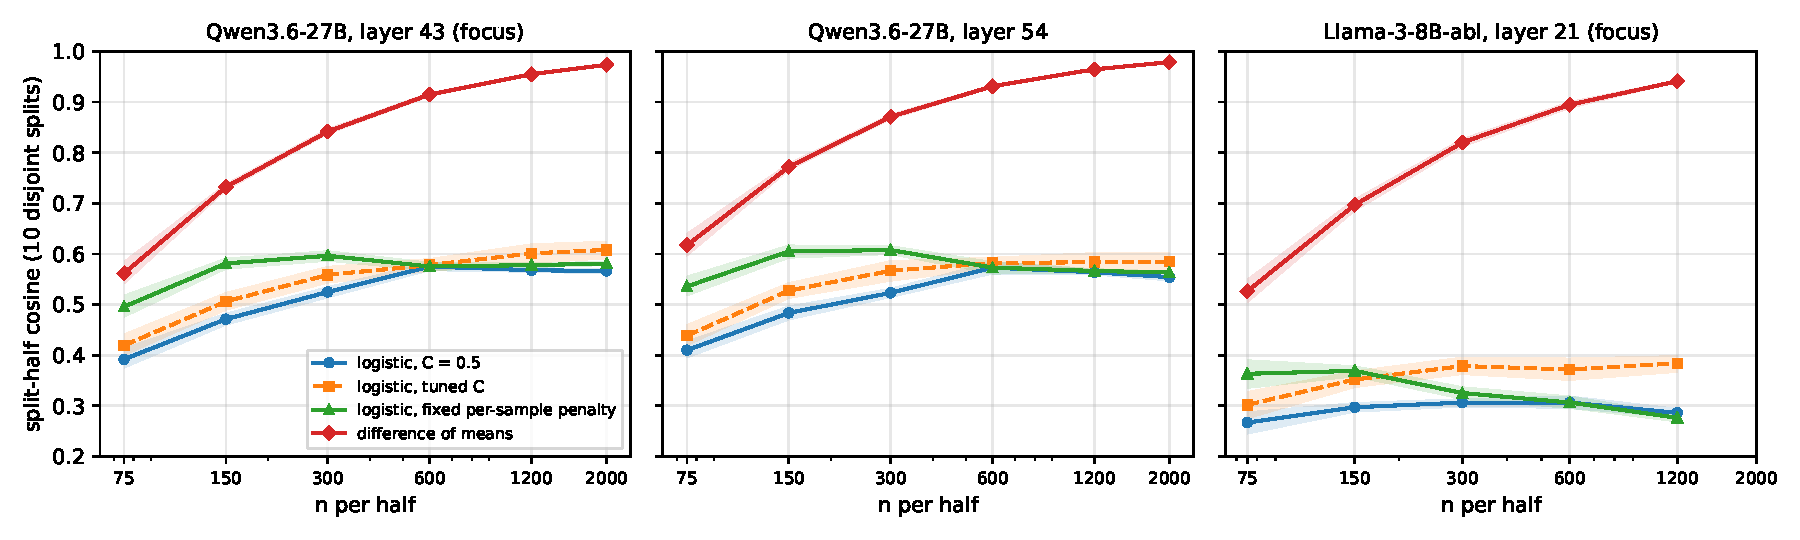
\includegraphics[width=0.72\linewidth]{fig1_splithalf_vs_n}
\caption{\textbf{Logistic directions do not reproduce; difference-of-means does.} Split-half cosine of the fitted direction over ten disjoint splits against $n$ per half, at two depths of the 27B and the focus layer of the 8B. Difference-of-means rises toward 1 with $n$; logistic at $C=0.5$ and at a fixed per-sample penalty (anchor 600) plateau near 0.55--0.6 (27B) and fall to 0.28--0.33 (8B); tuned $C$ reaches 0.61 and 0.38. Bands are bootstrap CIs over splits.}
\label{fig:splithalf}\end{figure}

\paragraph{Disjoint-half reproducibility.} We fit the same estimator on two disjoint halves of $n$ items each, ten independent splits, and report the mean per-class cosine between the two fitted directions (Figure~\ref{fig:splithalf}). At the 27B focus layer with $n=2000$ per half, difference-of-means reaches 0.974 and logistic regression ($C=0.5$) 0.566 (\rid{a2.focus\_dom\_split\_half}, \rid{a2.focus\_logreg\_split\_half}); at layer 54, 0.979 against 0.554 (\rid{a2f54.*}); on the 8B focus layer at $n=1200$, 0.941 against 0.286 (\rid{a2\_8b.*}). Tuning $C$ per fit by cross-validation reaches 0.61 on the 27B (\rid{a2f.focus\_tuned\_c\_does\_not\_close\_gap}) and 0.38 at the 8B focus layer (0.37--0.41 across three depths; \rid{a2f8.lam\_declines}, note).

\paragraph{Holding the per-sample penalty fixed does not help.} A natural objection is that a fixed $C$ changes the effective penalty as $n$ grows. With $C_n = 0.5\,N_{\mathrm{ref}}/n$, so that the per-sample penalty is constant, the logistic curve shows no net rise from $n=150$ to $2000$ at two anchors on the 27B focus layer (0.581 at both ends for the 600 anchor; a dip at 600 of $-0.021$ that is significant in a paired test over the ten shared splits, 1 of 10 positive, and a partial recovery; \rid{a2f.focus\_logreg\_fixed\_lambda\_flat}, \rid{a2f2.lam\_anchor2000\_no\_rise}), one drop at 300$\to$600 and then flat at layer 54 (\rid{a2f54.lam\_declines\_anchor600}), a rise at layer 16, and on the 8B a peak at 150 followed by a fall to 0.276 at 1200 (\rid{a2f8.lam\_declines}). The picture is depth-specific, with no convergence over the reachable range ($n \le 2000$, $d = 5120$ on the 27B, a 27-fold increase in $n$; $n \le 1200$, $d = 4096$ on the 8B): a proportional-regime statement, not an asymptotic one.

\begin{figure}[t]\centering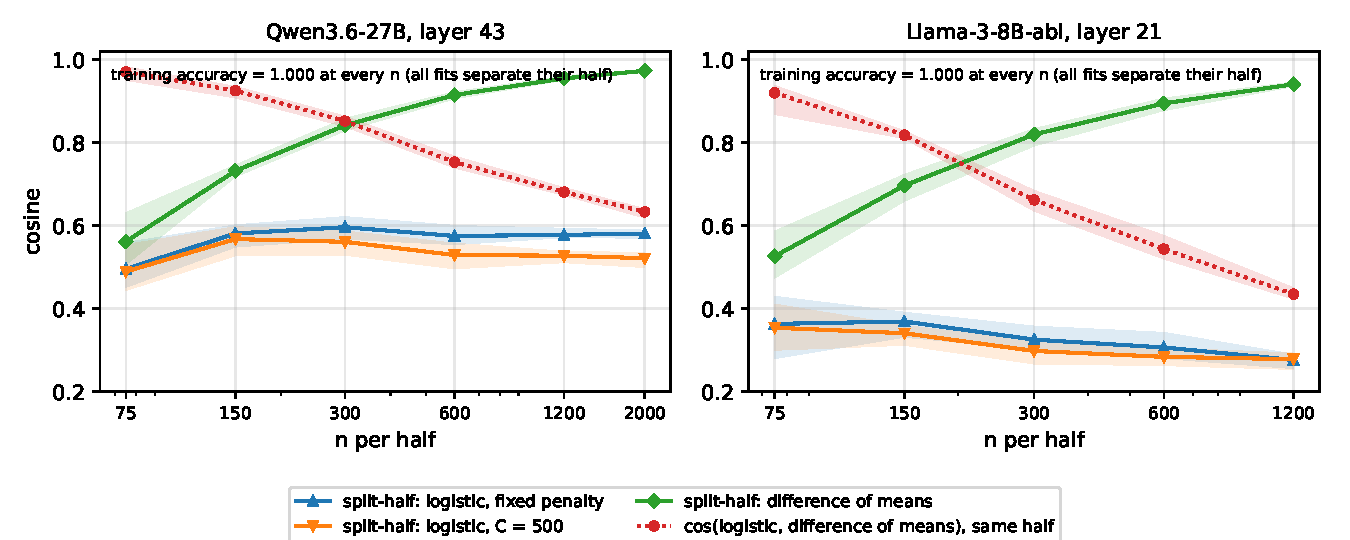
\includegraphics[width=0.66\linewidth]{fig2_margin_divergence}
\caption{\textbf{The logistic direction is a separator's tie-break that drifts away from the mean difference.} Within one half, the cosine between the fixed-penalty logistic direction and the difference-of-means direction falls as $n$ grows, while difference-of-means becomes reproducible across halves and the logistic direction does not, under the fixed schedule (anchor 600) or a thousandfold weaker penalty ($C=500$) alike. Every fit has training accuracy 1.000.}
\label{fig:margin}\end{figure}

\paragraph{Why.} Every multinomial logistic fit on every half at every $n$ used, under the fixed schedule and $C = 0.5$, 50 and 500 alike (the two weak arms being one tolerance-limited solution), separates its training half perfectly: accuracy exactly 1.000 in every cell, arm and seed; worst single-fit log-loss 0.0055; at most 80 iterations (\rid{a2m.separable\_every\_n}, \rid{a2m.8b\_same\_regime}, \rid{a2m.v2\_ten\_seeds}). The likelihood is saturated from $n=75$: the direction is the penalty's tie-break among separating hyperplanes. Weakening the penalty a hundredfold or a thousandfold leaves the direction unchanged on the same half (cosine $\ge 0.96$) and no more reproducible (0.52 against 0.58 at $n=2000$; \rid{a2m.weak\_penalty\_same\_direction}). The separator starts near the mean-difference direction and departs from it as $n$ grows, cosine 0.97$\to$0.63 on the 27B (\rid{a2m.logistic\_departs\_from\_dom}) and 0.91$\to$0.43 on the 8B (\rid{a2m.8b\_same\_regime}), while difference-of-means becomes reproducible (Figure~\ref{fig:margin}). In these units difference-of-means is the raw-space direction $(\mu_+-\mu_-)/\sigma^2$; the plain mean difference $\mu_+-\mu_-$ that contrastive activation addition uses agrees with the logistic direction at 0.43 (27B) and 0.33--0.37 (8B) (\rid{a2f.caa\_raw\_vs\_logreg\_raw}, \rid{a2f8.cross\_estimator}), against the 0.98--0.99 that \citet{herbster2026steering} report for compassion. Not claimed: that the fit sits at the max-margin limit (the weak arms are tolerance-limited), or a support-vector mechanism for the drift.

\paragraph{Is this just $n<d$, and does it cost anything?} Separation is guaranteed for generic data whenever $n<d$, so the mechanism is regime-conditional and the paper's recommendation holds because probe pools in this literature are small relative to model width. Three checks bound what this means. On held-out items at the 27B focus layer the logistic probe decodes \emph{better} than difference-of-means (six-way accuracy 0.82 to 0.94 against 0.79 to 0.88 at $n=75$ to $2000$), and the two estimators' projections of the same held-out items correlate at 0.96 to 0.90 over the same range (\rid{a2l.heldout\_and\_projcorr}): the coefficient row is a fine classifier and a poor direction, the dissociation \citet{marks2023geometry} described, and the instability is largely geometric. Projecting the activations onto their top 100 principal components and refitting shows the regime dependence directly: with $n/d'$ up to 20 the fits stop separating their halves from $n=600$ (training accuracy 0.999, 0.989, 0.974 at $n = 600$, 1200, 2000), the logistic direction becomes reproducible (0.90 at $n=2000$ in standardised coordinates against 0.94 for difference-of-means, from 0.39 and 0.33 at $n=75$), and its cosine to the difference-of-means direction stays at 0.91--0.94 across $n$ instead of falling from 0.90 to 0.62 as it does at full width (these are standardised-coordinate cosines; the 0.97$\to$0.63 above is the raw-space convention of Figure~\ref{fig:margin}); held-out accuracy in 100 dimensions is 0.92 against 0.94 at full width (\rid{a2l.lowd\_recovers}). The 8B behaves the same way: in 100 dimensions training accuracy falls to 0.90 at $n=1200$ and the logistic direction reproduces at 0.81 against 0.85 for difference-of-means (\rid{a2l.8b\_lowd}). The mechanism is therefore the $n<d$ regime itself, and the recommendation holds because probe pools in this literature are small relative to model width.

\section{The receiver's response}
\label{sec:transfer}
\begin{figure}[t]\centering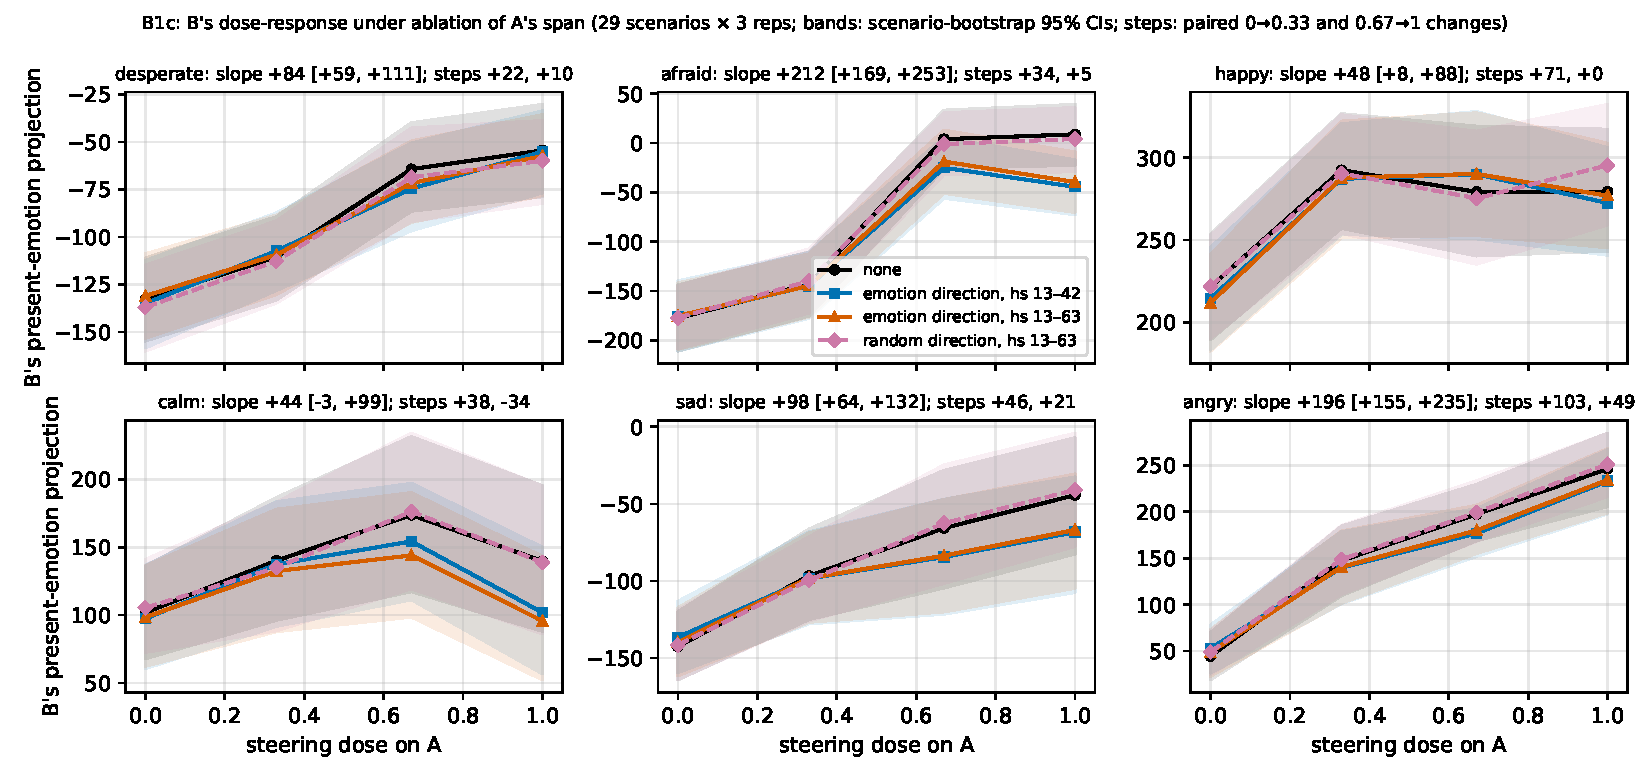
\includegraphics[width=0.62\linewidth]{fig3_b1c_dose_response}
\caption{\textbf{The projection responds to steering; two of six responses are not monotone, and the ablation arms separate from baseline to significance for afraid and sad only among the testable emotions.} B's present-emotion projection against A's steering dose, per emotion, under no ablation and under the three ablation arms of B1c (29 scenarios $\times$ 3 replicates; bands are scenario-bootstrap 95\% intervals of the per-dose mean). Titles give the none-arm slope with its CI and the paired changes over the first and last dose steps. Happy saturates after the first step and calm reverses at the top dose; calm's separation is the largest in the figure but calm is untestable. Between-arm separation is decided by the paired contrasts of Tables~\ref{tab:decision}--\ref{tab:arms}, not by the drawn bands, which are per-arm.}
\label{fig:dose}\end{figure}
B's present-emotion projection rises with A's dose for desperate, afraid, happy, sad and angry, with none-arm slopes from $+48$ to $+212$ and CIs excluding zero; calm's ($+44$ $[-3, +99]$) does not, so calm is untestable under the pre-registered rule (\rid{b1c.verdict\_H1}; Figure~\ref{fig:dose}). The slope is a poor summary for two emotions: happy rises $+71$ $[+50, +94]$ over the first dose step and $+0$ $[-24, +25]$ over the last, calm $+38$ $[-3, +78]$ then $-34$ $[-77, +13]$, while desperate, sad and angry rise at both steps (\rid{rev.dose\_shape}). The B1 follow-up run, with independently sampled replies, gives the same five testable emotions and afraid/sad as the blocked ones (\rid{b1f.*}); B1c--B1e share pool, directions and seeds and agree bit for bit on shared arms, a determinism check rather than a replication (\rid{b1d.replicates\_b1c\_arms}). The manipulation check on A passes for all six emotions in each run. On the 8B the same five emotions respond (\rid{b1c8.transfer\_replicates}), with a steering manipulation half as strong and less specific, so only the pattern is compared.

\paragraph{What the probe measures.} B's other-speaker projection, the matching probe for the interlocutor's emotion, rises with A's dose as well: slopes $+59$, $+119$, $+65$, $+93$, $+96$ for desperate, afraid, happy, sad and angry against present-probe slopes $+84$, $+212$, $+48$, $+98$, $+196$ (\rid{rev.other\_probe\_rises}). The present-emotion projection therefore does not separate B's own state from B's representation of A's, and we make no claim about which it is; an earlier claim that the present shift exceeds the other did not survive a non-circular probe (report 18 in the repository).

\section{Three pre-registered ablations}
\label{sec:ablations}
All directions are fitted per layer on the DIR half: the emotion direction at each hidden state 13--63 is that layer's own difference-of-means direction; ``readable'' means the layer passes the pre-registered split-half gate ($\ge 0.80$), which every layer from 13 upward does and the window starts at $0.2\times$ depth by design.

\begin{table}[t]\centering\footnotesize
\caption{Pre-registered decision contrasts, as blocked fractions of the none-arm slope (B1c: emotion direction $-$ random direction; B1d: affect subspace $-$ permuted-label subspace; B1e: emotion direction $-$ permuted-label direction). $^{*}$: BH-FDR $q<0.05$ within the contrast's own family of five testable emotions; $^{\cdot}$: unadjusted CI excludes zero only. Calm ($u$) is untestable.}
\label{tab:decision}
\begin{tabular}{lcccccc}\toprule
 & desperate & afraid & happy & calm$^{u}$ & sad & angry \\ \midrule
B1c: emotion dir $-$ random dir & 0.06 & 0.21$^{*}$ & 0.05 & (0.94)$^{\cdot}$ & 0.33$^{*}$ & 0.09 \\
B1d: affect subspace $-$ permuted subspace & 0.14 & $-$0.13$^{\cdot}$ & 0.05 & (1.56)$^{\cdot}$ & 0.26$^{\cdot}$ & 0.17$^{\cdot}$ \\
B1e: emotion dir $-$ permuted-label dir & 0.06 & 0.25$^{*}$ & $-$0.14 & (1.02)$^{\cdot}$ & 0.29$^{*}$ & 0.09 \\ \bottomrule
\end{tabular}
\end{table}

\begin{table}[t]\centering\footnotesize
\caption{Every hooked arm against baseline (none), as blocked fractions of the none-arm slope, scenario-blocked and dose-paired; marks as in Table~\ref{tab:decision}, families being the arm's five testable emotions (\rid{rev.b1c\_random\_vs\_none}, \rid{rev.b1c\_emo\_vs\_none\_fdr}, \rid{rev.b1d\_controls\_vs\_none}).}
\label{tab:arms}
\begin{tabular}{llcccccc}\toprule
run & arm $-$ none & desperate & afraid & happy & calm$^{u}$ & sad & angry \\ \midrule
B1c & emotion direction (rank 1, hs 13--63) & +0.08 & +0.24$^{*}$ & -0.24 & (+0.98)$^{\cdot}$ & +0.28$^{\cdot}$ & +0.09 \\
B1c & emotion direction (rank 1, hs 13--42) & +0.03 & +0.27$^{*}$ & -0.11 & (+0.79)$^{\cdot}$ & +0.33$^{*}$ & +0.12$^{*}$ \\
B1c & random direction (rank 1) & +0.02 & +0.03 & -0.28 & (+0.04) & -0.04 & -0.00 \\
B1d & affect subspace (rank 5) & +0.16 & +0.11$^{\cdot}$ & -0.05 & (+1.32)$^{\cdot}$ & +0.54$^{*}$ & +0.40$^{*}$ \\
B1d & permuted-label subspace (rank 5) & +0.03 & +0.23$^{*}$ & -0.10 & (-0.24) & +0.27$^{*}$ & +0.23$^{*}$ \\
B1d & random 5-frame (rank 5) & +0.05 & +0.02 & -0.17 & (-0.12) & -0.01 & +0.06 \\
B1d & random 23-frame, footprint-matched (rank 23) & +0.06 & -0.03 & +0.03 & (+0.68)$^{\cdot}$ & +0.07 & +0.00 \\
B1e & permuted-label direction (rank 1) & +0.02 & -0.00 & -0.10 & (-0.04) & -0.01 & +0.00 \\
B1e & top principal direction (rank 1) & +0.16 & -0.01 & +0.30 & (+0.98)$^{\cdot}$ & -0.13 & +0.61$^{*}$ \\
\bottomrule\end{tabular}
\end{table}

\begin{table}[t]\centering\footnotesize
\caption{The directions and frames: rank; footprint (norm removed per masked position, averaged over ablated layers) with its ratio to the emotion direction in the same run; largest dose-0 shift of the A-span readout; share of readable affect removed at the top dose (range over emotions). $^{\dagger}$: the 23-frame's run has no emotion arm; its ratio uses the B1d run's emotion direction, and the two runs' none arms agree bit for bit (\rid{b1d23.footprint\_matched}). (\rid{b1c.random\_control\_inert}, \rid{b1d.footprint}, \rid{b1e.verdict\_H3}, \rid{b1e.pc1\_dissociation}, \rid{rev.b1d\_controls\_vs\_none})}
\label{tab:dirs}
\begin{tabular}{llcccc}\toprule
run & arm & rank & footprint (ratio) & dose-0 shift & readable affect removed \\ \midrule
B1c & emotion direction & 1 & 0.46--0.66 (1) & $\le 0.01$ & 0.16--0.79 \\
B1c & random direction & 1 & 1.15--1.26 (2.0) & $\le 0.01$ & $\le 0.03$ \\
B1d & affect subspace & 5 & 6.9 (10.5) & $+0.39$ / $-0.25$ & 0.11--1.25 \\
B1d & permuted-label subspace & 5 & 6.5--6.9 (10) & $\le 0.08$ & 0.07--0.52 \\
B1d & random 5-frame & 5 & 3.1--3.2 (5) & $\le 0.01$ & $\le 0.03$ \\
B1d & random 23-frame, footprint-matched & 23 & 6.7--6.9 (10)$^{\dagger}$ & $\le 0.01$ & $\le 0.13$ \\
B1e & permuted-label direction & 1 & 0.50 (0.85; afraid 0.84, sad 0.77) & $\le 0.01$ & $\le 0.09$ \\
B1e & top principal direction & 1 & 3.47 (5.8) & $+0.55$ / $-0.28$ & 0.71--1.5 \\ \bottomrule
\end{tabular}
\end{table}

\begin{figure}[t]\centering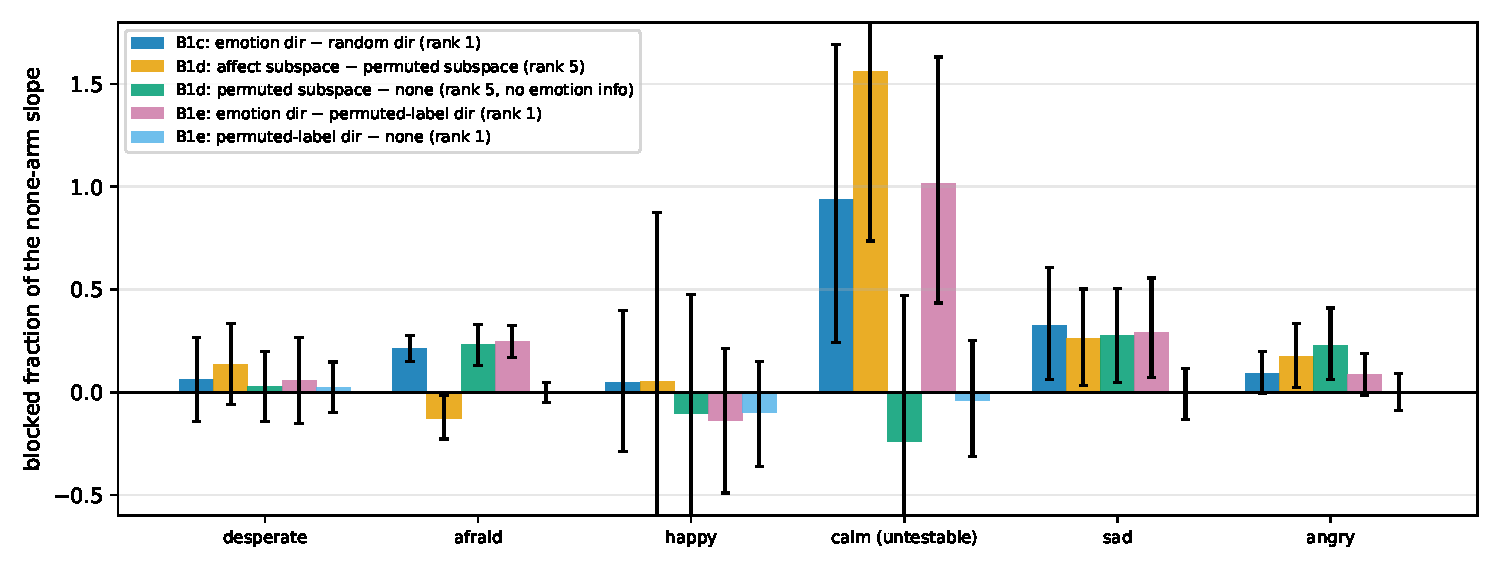
\includegraphics[width=0.74\linewidth]{fig4_blocked_fractions}
\caption{\textbf{Every arm against baseline: which ablations block, and which controls bite.} Blocked fraction of the none-arm slope for every hooked arm of the three 27B experiments (Table~\ref{tab:arms}). The permuted-label rank-5 subspace blocks afraid, sad and angry at BH-FDR $q<0.05$; the random direction, the random 5-frame and the permuted-label rank-1 direction block nothing; the top principal direction blocks angry. Error bars are CI-implied ranges (the contrast's confidence interval divided by the none-arm slope, re-sorted); calm's bars and happy's lower whiskers are clipped at the axis.}
\label{fig:blocked}\end{figure}

\paragraph{B1c: the rank-1 direction (verdict H1).} Projecting the difference-of-means emotion direction out of A's span at every hidden state 13--63 during B's prefill removes, against the random-direction control, a median 9\% of the dose-response over the five testable emotions (scenario-bootstrap CI of the median $[4\%, 25\%]$; the per-emotion values are 0.06, 0.21, 0.05, 0.33, 0.09, and the median with calm included is 15\%; \rid{b1c.verdict\_H1}, \rid{b1c.median\_fraction}, \rid{rev.b1c\_emo\_vs\_none\_fdr}). Against baseline the median is 9\% (17\% with calm). Afraid (21\%, $q=0.001$) and sad (33\%, $q=0.048$) are the only blocks that clear the false-discovery rule against the random control; against baseline afraid clears ($q=0.001$) and sad does not ($q=0.115$) (\rid{b1c.partial\_block\_replicates}). Extending the ablation to layers 43--63 changes no dose-response detectably, with the extra blocking bounded under 0.08 for afraid, angry, happy and sad (a driver-declared contrast; \rid{b1c.no\_gain\_beyond\_layer42}). The unit-norm random direction, removing twice the norm, is inert against baseline for all six emotions (largest happy $+13.5$ $[-0.1, +28.4]$, $q \ge 0.26$; \rid{rev.b1c\_random\_vs\_none}). Across the five testable emotions the blocked fraction rises with the share of readable affect the ablation removes ($r \approx 0.85$ on five points, $p \approx 0.07$, descriptive; \rid{b1c.readout\_residual}): the rank-1 direction is insufficient to carry the response.

\paragraph{B1d: the rank-5 subspace (verdict instrument\_failed).} Projecting out the rank-5 class-mean affect subspace (16--21\% of the pool's variance; \rid{b1d.frame\_geometry}) removes at least 80\% of the readable affect for only three of six emotions and shifts the readout at dose 0 (desperate 0.11$\to$0.50; \rid{b1d.readout\_baseline\_shift}): the instrument and the ablation share a target, and the pre-registered decision is void. Against baseline (Table~\ref{tab:arms}) the affect subspace blocks sad (54\%) and angry (40\%) at $q=0.001$; a permuted-label subspace built by the same estimator, with no emotion information and a third of its span in common with the affect frame, blocks afraid (23\%), sad (27\%) and angry (23\%) at $q = 0.001$, 0.035 and 0.013 (\rid{b1d.perm\_control\_blocks}, \rid{rev.b1d\_controls\_vs\_none}), with dose-0 readout shifts below 0.08; a random 5-frame with half its footprint blocks nothing ($q \ge 0.51$), and neither does a random 23-frame matched to the permuted frame's footprint (6.7--6.9 against 6.5--6.9 per position; blocked fractions $-0.03$ to $+0.07$, $q \ge 0.71$; \rid{b1d23.inert}, \rid{b1d23.footprint\_matched}). The pre-registered contrast, affect minus permuted subspace, clears no false-discovery threshold ($q=0.051$; \rid{b1d.median\_fraction\_descriptive}); the affect subspace differs from the rank-1 direction in opposite directions (afraid $+29.3$ slope units, i.e.\ less blocking; angry $-60.6$, more; \rid{b1d.rank5\_vs\_rank1}).

\paragraph{B1e: a permuted-label rank-1 control (verdict H3).} The same estimator on permuted labels gives a rank-1 direction with cosine 0.004 to the emotion direction (Appendix~\ref{app:details}) and 0.85$\times$ its footprint on average (0.84 afraid, 0.77 sad); removed at all 51 layers it changes no emotion's dose-response and removes no readable affect (\rid{b1e.permdir\_inert}). Against it the emotion direction blocks afraid by 25\% $[17\%, 33\%]$ and sad by 29\% $[7\%, 56\%]$ (BH-FDR $q$ 0.001 and 0.028; \rid{b1e.verdict\_H3}); the corresponding blocks against baseline are 24\% and 28\%. Ten re-splits of the probe pool, each re-estimating every direction and the readout probe (Table~\ref{tab:draws}), put that draw at the top of afraid's spread and inside sad's: afraid's block is 18\% at the median (7--23\%), significant in nine draws, but its manipulation check (the A-span readout's response to A's own steering) passes in only four, so the verdict is H3 in four draws and instrument\_failed in six; sad's is 35\% (24--56\%), significant in all ten with the check passing in all ten; the permuted direction stays within 7\% (afraid) and 13\% (sad) of baseline throughout (\rid{b1e10.sad\_stable}, \rid{b1e10.afraid\_gate\_fragile}). The top principal direction of A's span, label-free and unfitted to labels, with 5.8$\times$ the footprint, blocks angry by 61\% ($q=0.001$) and calm (untestable) while leaving afraid and sad untouched though it removes 79\% and 71\% of their readable affect, and shifts the dose-0 readout by up to 0.55 (\rid{b1e.pc1\_dissociation}): readable-affect removal and blocking dissociate. B1d's rank-5 permuted frame blocks where B1e's rank-1 permuted direction does not; they differ in rank and in footprint (10$\times$ against 0.85$\times$). Footprint alone is ruled out by the matched random 23-frame, which removes as much and blocks nothing (\rid{b1d23.inert}): the arms that block (affect subspace, permuted-label frame, top principal direction) are all estimated from the pool's activations, and the inert ones are not. The secondary readout on B's reply agrees for sad and not for afraid (Appendix~\ref{app:details}).

\paragraph{Replication on the 8B.} B1c's design blocks the same two emotions on the 8B by unadjusted CIs (afraid 15\%, sad 31\% against the random direction; \rid{b1c8.verdict\_and\_block}), the other three too wide to tell; its manipulation-check rule returned instrument\_failed because the upper window changes the readout by nothing measurable there and the strict criterion has no tolerance band. B1e's design returns H3 on the 8B (sad 36\%, $q$ 0.002, secondary readout agreeing; afraid 14\%, $q$ 0.08, no block against baseline), but the control is matched only on average and B1c's random direction reproduced the contrasts there, so the run adds no discriminating power. Only sad replicates across models on both outcomes (\rid{b1e8.verdict\_H3\_matched}).

\section{What the controls teach}
\label{sec:controls}
Table~\ref{tab:arms} puts every arm on one scale (the CI-implied range is the contrast's interval divided by the none-arm slope). The random direction, the random 5-frame and the permuted-label rank-1 direction are inert; the permuted-label rank-5 frame blocks three emotions at the false-discovery threshold, as strongly as the affect subspace blocks two of them; the top principal direction blocks a different one. A study with only the random control would have called B1d's blocks emotion-specific. A random frame scaled to the permuted frame's footprint (rank 23) is inert (\rid{b1d23.inert}), so matching a control's footprint is not enough; the control must be fitted by the intervention's own estimator. The rule is procedural: beside the random direction, run the same estimator on permuted labels at the intervention's rank, report every arm's footprint and dose-0 readout shift, and check the manipulation with an instrument that does not share the ablation's target.

\section{Limitations and what is not claimed}
\label{sec:limits}
The present-emotion projection does not separate B's own state from B's representation of A's; the other-speaker projection moves comparably. One probe pool underlies all 27B ablations; the direction's sampling variability is measured by ten re-splits for B1e's two emotions only (Table~\ref{tab:draws}), not for B1c or B1d, and afraid's manipulation check is split-sensitive. The A-span readout is forced-choice and shares a target with the subspace ablation. The dose-response slope summarises a saturating curve for happy and afraid and a reversing one for calm. All intervals are percentile bootstraps over 29 scenario clusters; multiplicity is controlled within experiments, not across the three experiments and two models. The estimator mechanism is regime-conditional ($n<d$). Recorded defects: Appendix~\ref{app:details}; seeds, hardware and software: Appendix~\ref{app:repro}. Not tested: the token channel (three rewrite designs failed their own manipulation check; \rid{b1c.text\_arms\_uninterpretable}), the behavioural reach, layers below 13, and an ablation rerun with the logistic direction.

\section{Conclusion}
\enlargethispage{4\baselineskip}
The idea to take away is that the two failures we found are the same failure seen twice. A logistic direction on separable activations is decided by the penalty's tie-break, so two independent fits agree only as far as their tie-breaks do; and a control direction is informative only if it is decided the way the intervention direction was. Random vectors are decided by nothing, which is why they are inert and miss what a fitted control catches. Such a study should report disjoint-half reproducibility, estimate with an average rather than an extremum, and run its ablations against a control fitted by the same estimator on permuted labels. For affect: the rank-1 direction carries a third of sad's response in every draw and on both models, and part of afraid's less reliably; whose state the probe reads remains open.

\appendix
\section{Reproducibility statement}
\label{app:repro}
Code, pre-registrations, result files and the claim registry are in the accompanying repository (research-use licence). Models: Qwen3.6-27B revision \texttt{6a9e13bd} and Llama-3-8B-Instruct-abliterated revision \texttt{dd67dd05}, run with torch 2.11.0+cu130 and transformers 5.14.1 on one NVIDIA RTX PRO 6000 (96\,GB) per run; a 27B ablation experiment takes about two hours (432 or 288 arm-rows of 29 scenarios each, 19--21\,s per arm-row), the 8B one under thirty minutes. Seeds: pool generation seed 0; per-generation seeds are a CRC32 of (seed, emotion, dose, replicate, arm, part) with the arm field empty for the receiver's reply so that arms share random numbers; ten split seeds (0--9) for every split-half number; bootstrap seed 0 with 5{,}000 draws. Two further 27B runs were added after review (2026-09-06, pre-registered as addenda to PREREG\_B1d and PREREG\_B1e before launch): ten B1e draws that re-split the same probe pool with split seeds 1--10 (the original run used 0), restricted to afraid and sad and the arms none, emotion direction and permuted-label direction, so that the steering direction, the per-layer ablation directions, the control and the readout probe are all re-estimated per draw; and one B1d run with the arms none and random frame only, the frame's rank raised from 5 to 23 so that its expected footprint matches the permuted-label frame's ($5 \times (6.7/3.15)^2 \approx 23$). Generation seeds, doses, replicates and scenarios are unchanged, so each draw's none arm is a fresh sample of the same design. Hyperparameters: doses $\{0, 0.33, 0.67, 1\}$ at a fixed activation-RMS scale, three replicates, 29 scenarios, 110 new tokens per message at temperature 0.9; logistic regression with lbfgs, max\_iter 3000, $C \in \{0.5,\ C_n = 0.5\,N_{\mathrm{ref}}/n \text{ with } N_{\mathrm{ref}} \in \{600, 2000\},\ 50,\ 500\}$ and cross-validated $C$ on a decade grid scored for accuracy; split-half $n \in \{75, 150, 300, 600, 1200, 2000\}$ per half where the pool allows. Statistics: scenario-blocked percentile bootstraps because scenarios are the sampling unit; between-arm contrasts paired within scenario and dose; two-sided bootstrap $p$-values with Benjamini--Hochberg over the testable emotions of one arm; every interval in the paper is such a bootstrap and every count of runs is stated. The probe pools and scenario lists are committed with the results.


\section{Details and defects recorded under review}
\label{app:details}
Each item below is in the registry note of the claim it qualifies.
\begin{itemize}\setlength\itemsep{1pt}
\item \emph{B1c.} The contrast between the 30-layer and 51-layer windows was declared in the driver, not in the pre-registration; its null is unpowered for desperate and calm. The testability rule (none-arm CI excludes zero) is pre-registered (PREREG\_B1c \S5). Calm's contrast is the largest and is excluded by that rule; medians are reported with and without it. Afraid's top-dose readout is non-monotone. The pre-registration stamp is empty because the driver resolved its path relative to the wrong directory; the document was on the machine one second before the run started, and its commit (\texttt{cc2dc32}, 19:22Z) precedes the run's start (19:32Z) in the repository history. The pool has 1,615 items against the registered 2,160; the false-discovery rate ran over five emotions rather than six.
\item \emph{B1d.} The permuted-label subspace removed only 6.5\% of afraid's readable affect and still blocked its response, so overlap with the readable-affect direction does not explain its blocking; recomputing the instrument share with each arm's own floor keeps three failures but changes which emotions fail. The median's confidence interval resamples scenarios only. The footprint-matched 23-frame was run after review with only the none and random arms; it shifts calm, the untestable emotion, by $-30$ $[-55, -4]$ slope units (calm's own slope is $+44$ $[-3, +99]$), reported in Table~\ref{tab:arms} in parentheses and outside the false-discovery family.
\item \emph{B1e.} The control removes less norm than the emotion direction and less than B1c's inert random direction (1.22), so it is a fitted label-free null, not a footprint-matched one. The rule tests the point fraction and sad's range starts at 0.07. The secondary readout on B's reply contradicts afraid's block and agrees for sad. The control's cosine to the emotion direction (0.004) was measured by the pre-launch verifier and is not stamped in the result file.
\item \emph{Direction draws.} The ten re-splits reuse the pool file under a per-draw tag; draw 4 ran on a different machine from draws 1--3 after a rebalancing, with the same seeds. Afraid's manipulation check is a CI rule on the A-span readout slope; in the six failing draws that slope is $-0.02$ to $+0.09$ with intervals that include zero, two of them by less than 0.01, so the verdict split (four H3, six instrument\_failed) is a property of the gate, not of the decision contrast, which is significantly negative in nine draws. The addendum attaches no verdict to the ensemble; the medians and ranges are descriptive. The permuted direction against baseline reaches significance in one of the twenty emotion-draws (afraid, draw 6, $+6.5\%$ of the slope removed).
\item \emph{8B replications.} Both are out-of-pre-registration replications (the documents name the 27B and its layers). The steering manipulation is half as strong and less specific on the 8B, afraid's readout sits below chance, and slopes are unnormalised probe scores, so only patterns are compared. In B1e on the 8B the control is matched on average only (sad 0.86$\times$), both directions remove about the isotropic norm, and B1c's random direction already reproduced the contrasts; afraid does not block against baseline there.
\item \emph{Estimator study.} The weak-penalty arms ($C = 50$ and $500$) give the same solution to three decimals, so they are tolerance-limited and bound nothing about the $C \to \infty$ limit. Cross-estimator cosines use subsamples that overlap by about half the pool, so their intervals overstate precision. The layer-43 and layer-54 files come from three driver builds; the shared cells agree bit for bit.
\end{itemize}

\begin{table}[h]\centering\footnotesize
\caption{Direction-resampling draws (PREREG\_B1e addendum 3): blocked fractions of the none-arm slope for afraid and sad in ten re-splits of the probe pool (split seeds 1--10; ``Draw 0'' is the run in Table~\ref{tab:decision}), with the median and range across draws, the number of draws whose contrast is significantly negative, and the number of draws in which the emotion's manipulation check (the A-span readout responds to A's own steering) passes (\rid{b1e10.*}).}
\label{tab:draws}
\begin{tabular}{llrrrrr}
\toprule
Emotion & Contrast & Draw 0 & Median & Range & Sig.\ neg. & Gate passes \\
\midrule
afraid & emotion $-$ permuted-label & 0.25 & 0.18 & [0.07, 0.23] & 9/10 & 4/10 \\
 & emotion $-$ none & 0.24 & 0.19 & [0.08, 0.23] & 10/10 &  \\
 & permuted-label $-$ none & 0.00 & 0.02 & [-0.04, 0.07] & 1/10 &  \\
sad & emotion $-$ permuted-label & 0.29 & 0.35 & [0.24, 0.56] & 10/10 & 10/10 \\
 & emotion $-$ none & 0.28 & 0.35 & [0.23, 0.44] & 10/10 &  \\
 & permuted-label $-$ none & -0.01 & -0.01 & [-0.13, 0.09] & 0/10 &  \\
\bottomrule
\end{tabular}

\end{table}

\bibliographystyle{plainnat}
\bibliography{references}
\end{document}
